%------------------------------------------------------------------------------
\section{Reviews of estimation approaches} \label{sec:rev}
%------------------------------------------------------------------------------

%------------------------------------------------------------------------------
\subsection{Nonconvex and nonsmooth GMM objective function}	
%------------------------------------------------------------------------------
To estimate the linear IV quantile regression model, we need to solve the moment
condition specified in Equation \ref{eq:moment2}.  One necessary condition for
identification is that $dim(\Psi(\Xb, \Zb)) > k_\Xb + k_\Db$ with $dim(\Xb) =
k_x$  and $dim(\Db) = k_d$.

For $\thetab = (\alphab, \betab)$ and $\{\Wb_i\}_{i=1}^n = \{(Y_i, \Db_i',
\Xb_i', \Zb_i')'\}_{i=1}^n$, let
\begin{align}
\gb_\tau(\Wb_i, \thetab) = (
\left( \tau - \I (Y_i  - \Db_i'\alphab - \Xb_i'\betab \leq 0)  \right)
\Psib(\Xb_i, \Zb_i)
\label{eq:gi}
\end{align}
The empirical moment condition specified in Equation \ref{eq:moment3} can be
written as
\begin{align}
\hat{\gb}_N(\thetab) = \frac{1}{n}\sum_{i=1}^n \gb_\tau(\Wb_i, \thetab)
\end{align}
We can estimate $\thetab_0$ by GMM as
\begin{align}
\widehat{\thetab} = \argmin_{\thetab \in \Theta} n \hat{\gb}_N' \Omegab_N
\hat{\gb}_N
\label{eq:gmm_original}
\end{align}
where $\Omegab_N$ is the GMM weighting matrix and it is usually set to be
\begin{align}
\Omegab_N = \left(
	\tau(1-\tau) \frac{1}{n}\sum_{i=1}^n\Psib_i \Psib_i'
\right)^{-1}
\end{align}

Due to the indicator function in Equation \ref{eq:gi}, the GMM objective
function is nonsmooth and nonconvex. See Figure \ref{fig:ivqreg_crit} for an
illustration. 

\begin{figure}[H]
\centering
\label{fig:ivqreg_crit}
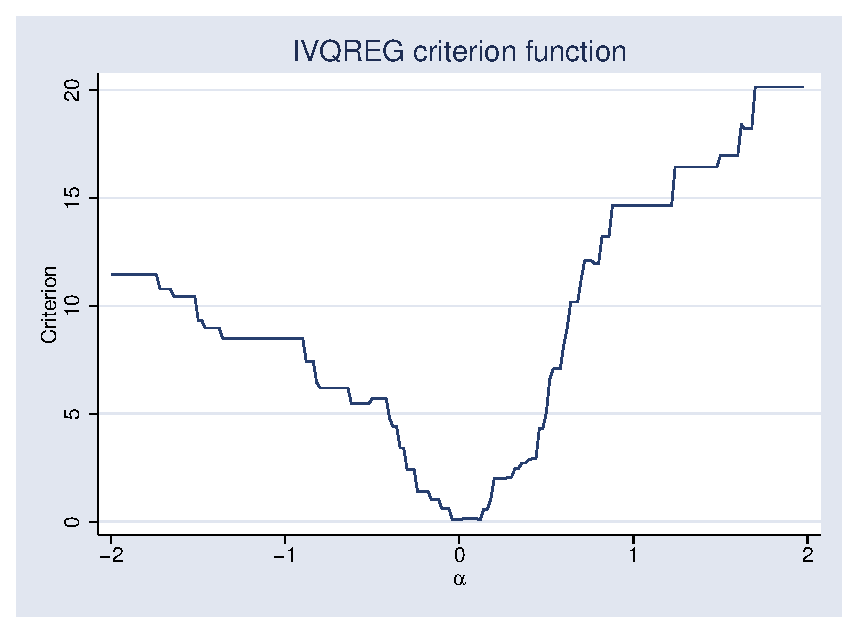
\includegraphics[scale=0.8]{eps/ivqreg_obj}
\caption{IVQREG GMM criterion function}
\end{figure}

For simplicity, the outcome variable only depends on one endogenous variable
$D$, and the true value of $\alpha$ equals to zero. We plot the GMM criterion
function at different values of $\alpha$. While the criterion function is
globally minimized at zero, the plot is flat in certain regions and exhibits
several local minimums. Thus, it is computationally difficult to solve the
optimization problem using the moment condition in Equation \ref{eq:moment3}.



%------------------------------------------------------------------------------
\subsection{Different approaches}	
%------------------------------------------------------------------------------

In literature, there are several estimation approaches to alleviate
the difficulties posed by non-smoothness and non-convexity. We list these
approaches in the chromatic order.

\begin{enumerate}
	\item \cite{Chernozhukov2003}: an MCMC approach.
	\item \cite{Chernozhukov2006}: inverse quantile regression
	\item \cite{Kaplan2017} and \cite{DeCastro2019}: smoothed estimating
	  equation
	\item \cite{Chen2018}: exact GMM via mixed-integer quadratic programming
	\item \cite{Kaido2021}: decentralization
\end{enumerate}

To avoid directly optimizing the original GMM optimization,
\cite{Chernozhukov2003} propose using the Markov Chain Monte Carlo method to
simulate the distribution of the parameter $\thetab$. We can implement this
approach using the {\tt bayesmh}. However, as usually seen in the Bayesian
approach, the estimator's performance may depend on other inputs such as prior
specification.  This method is worth implementation, or at least internally.  It
is interesting to compare the performance of this MCMC method with other
frequentist approaches.

\cite{Chernozhukov2006} propose estimating the IVQR model by conducting a
series of regular quantile regressions, and they name this method as inverse
quantile regression. This method is easy to implement but suffers from the curse
of dimensionality. The inverse quantile regression needs to do a grid search of
dimension $R^{k_d}$. However, this method can efficiently produce estimates at
different quantiles when there are a few endogenous variables. This method should
be implemented as a benchmark because it is already widely used.

\cite{Kaplan2017} and \cite{DeCastro2019} suggest to smooth the indicator
function in Equation \ref{eq:moment3} and then to solve the smoothed GMM
objective function. This method makes the objective function smooth, but the
non-convexity is still there. Thus, to implement this method, we need an
efficient optimization algorithm such as simulated annealing for the nonconvex
problem in Stata. We can use the Mata function {\tt solvenl()} to solve the
estimating equation for the just-identified case.  Compared with the inverse
quantile regression, the main advantage of this method  is that it does not
suffer from the curse of dimensionality. By the way, the over-identified case
can be transformed into a just-identified case by linear projection.

The recent advances of mixed-integer quadratic programming make it possible to
directly solve the nonconvex and nonsmooth optimization problems like Equation
\ref{eq:gmm_original}. \cite{Chen2018} show how to solve the original
GMM objective function in this path. This approach depends on the third-party
package for the mixed-integer quadratic programming algorithm.  Furthermore, 
this method is slow even when the sample size is moderate. 
Given the difficulty of implementing Stata's own mixed-integer quadratic
programming algorithm, we should not implement this method.

Finally, \cite{Kaido2021} propose recasting the original IVQR GMM
optimization problem into an iterative series of regular quantile regression.
The idea is to divide the problem into a simple and easy-to-compute subproblem,
denoting decentralization. The standard errors are obtained via
standard bootstrap. This method is promising because it is easy to implement as
the inverse quantile regression, and it does not suffer from the curse of
dimensionality. Furthermore, this method does not need extra tuning parameters
such as priors in the MCMC approach or the bandwidth choice in the smoothed GMM
approach.  However, this method requires adding the {\tt noconstant} option to
{\tt qreg}. Also, some preliminary simulation results show that this method is
sensitive to the starting values, and it may even be inconsistent when the model
is over-identified.

Considering the different properties of the above approaches, we propose the
following priority order of implementation.

\begin{enumerate}

\item Inverse quantile regression (benchmark)

\item Smoothed EE 

\item Decentralization (postpone due to {\tt noconstant qreg} and
over-identification issues)

\item MCMC approach (postpone)

\end{enumerate}

Section \ref{sec:iqr_method} describes the inverse quantile regression
estimator.  Section \ref{sec:see_method} introduces the smoothed EE estimator.
Finally, section \ref{sec:dec_method} documents the decentralized estimator.

